\section{Task 6}

\subsection{Overview of trigonometric interpolation}

Trigonometric interpolation approximates periodic functions with trigonometric polynomials. Its complexity is \( O(n \cdot m) \), where \( n \) is the number of interpolation points (\( n = 2m \)) and \( m \) is the number of polynomial coefficients. It uses periodic function values at evenly spaced nodes to determine the approximation coefficients.

The experiment examined how interpolation error changes with the number of points \( m \), and how well the algorithm reproduces selected continuous and discontinuous functions. Results are plotted below. Settings were as in Task 3/4.


\subsection{Results and conclusions}

\begin{center}
\textbf{Results for \( \sin(x) + \cos(x) \):}
Minimum error: \( 2.22e-16 \),
achieved for \( m = 3 \).
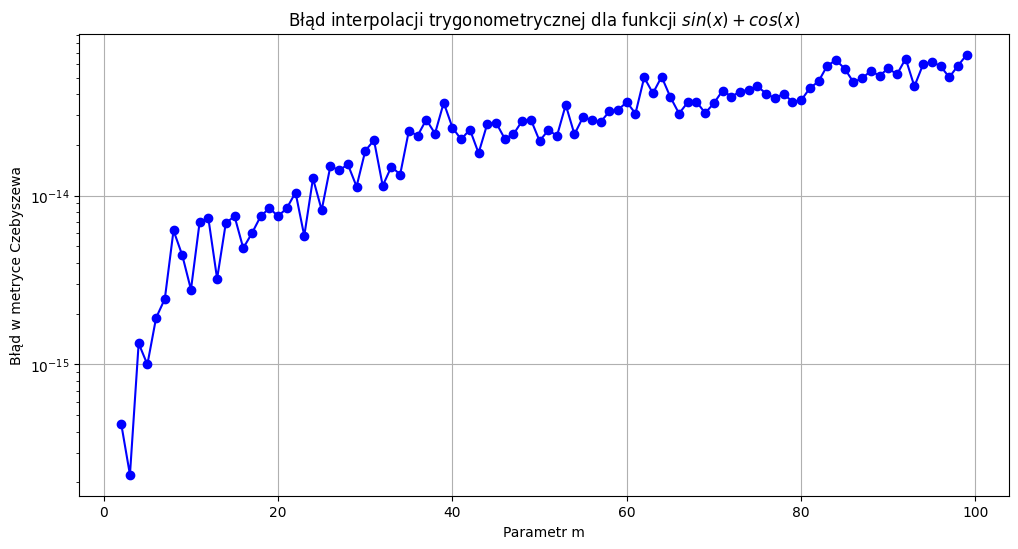
\includegraphics[width=0.8\textwidth]{figures/task-5/trigonometric_error.png}
\end{center}

\begin{minipage}{0.49\textwidth}
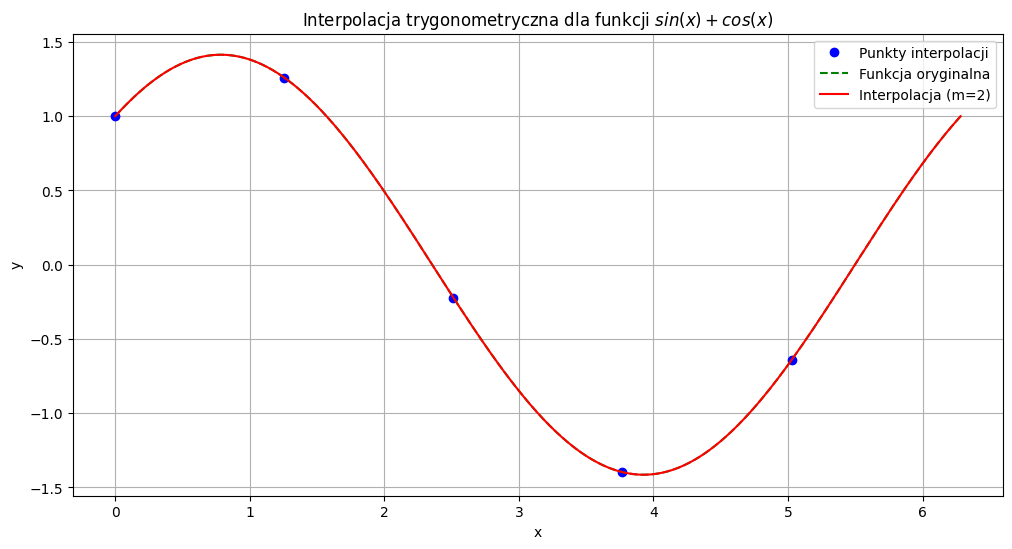
\includegraphics[width=\textwidth]{figures/task-5/trigonometric_2.png}
\end{minipage}
\begin{minipage}{0.49\textwidth}
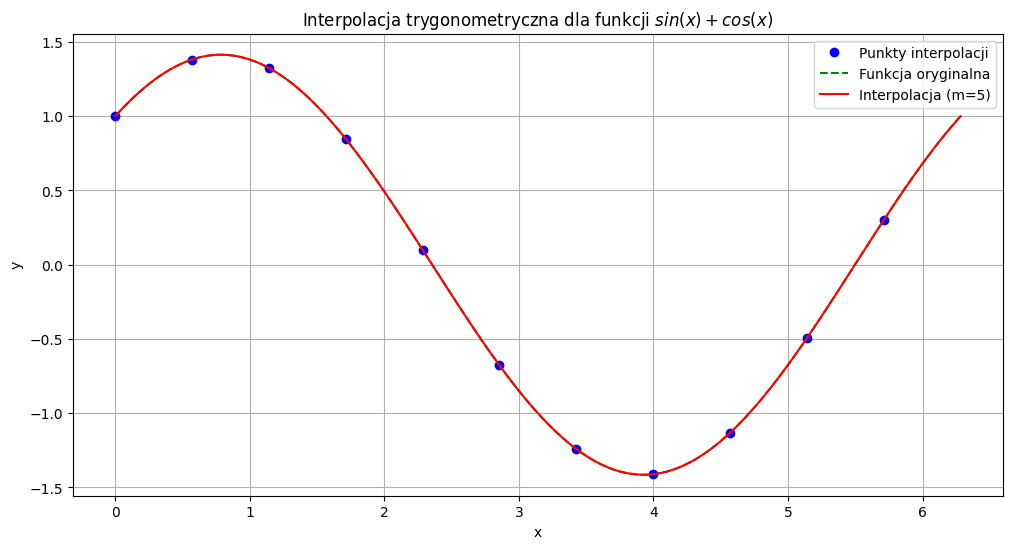
\includegraphics[width=\textwidth]{figures/task-5/trigonometric_5.png}
\end{minipage}

\begin{minipage}{0.49\textwidth}
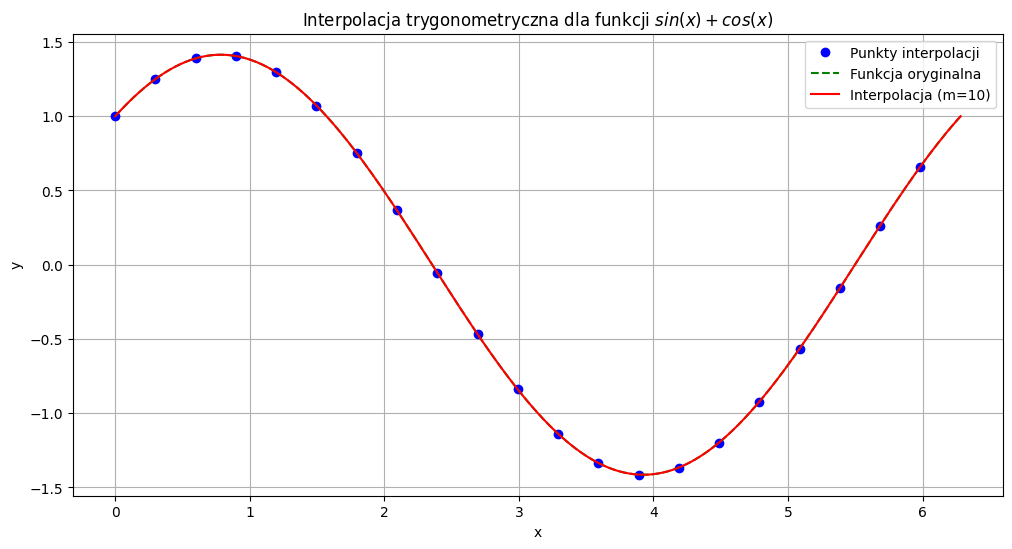
\includegraphics[width=\textwidth]{figures/task-5/trigonometric_10.png}
\end{minipage}
\begin{minipage}{0.49\textwidth}
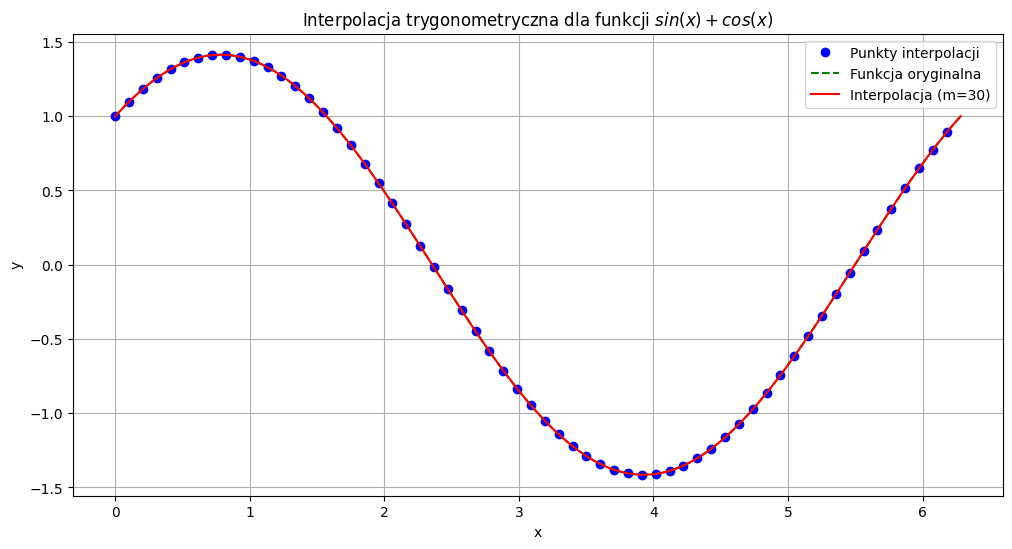
\includegraphics[width=\textwidth]{figures/task-5/trigonometric_30.png}
\end{minipage}

\begin{center}
\textbf{Results for \( \frac{1}{1+x^2} \):}
Minimum error: \( 9.75e-01 \),
achieved for \( m = 89 \).
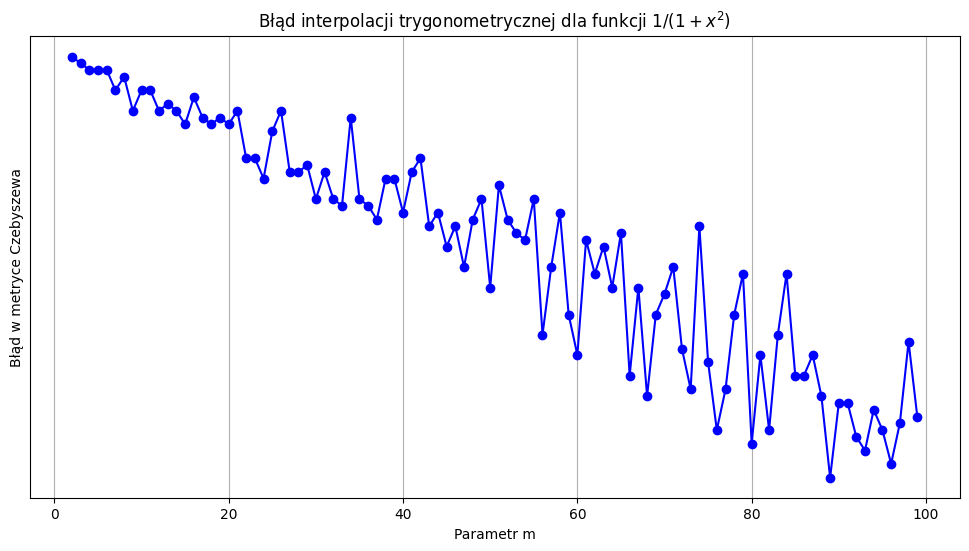
\includegraphics[width=0.8\textwidth]{figures/task-5/rational_error.png}
\end{center}

\begin{minipage}{0.49\textwidth}
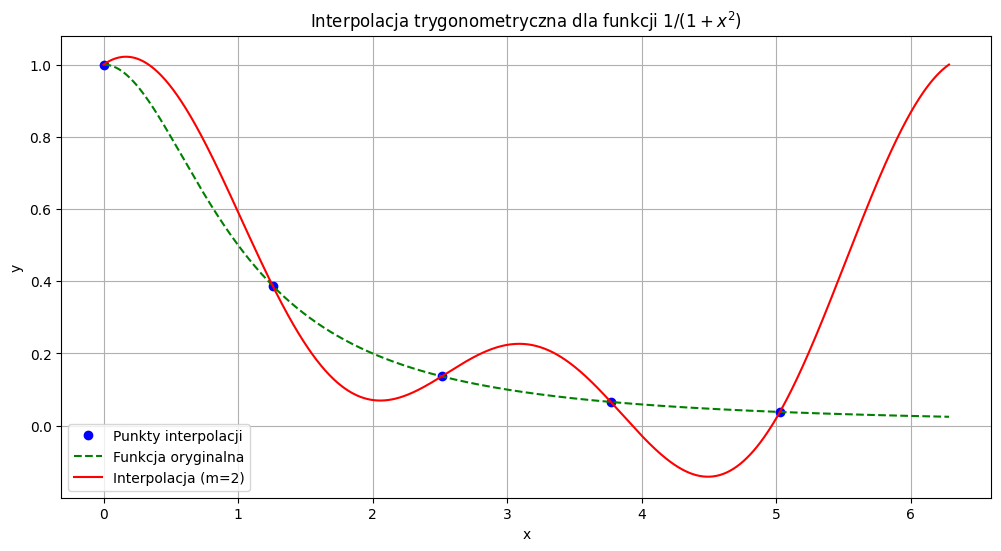
\includegraphics[width=\textwidth]{figures/task-5/rational_2.png}
\end{minipage}
\begin{minipage}{0.49\textwidth}
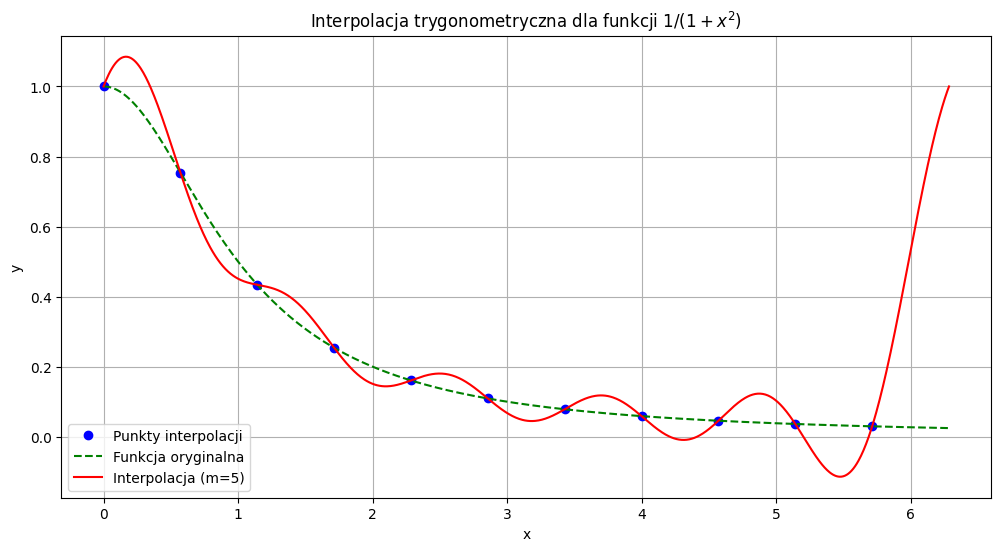
\includegraphics[width=\textwidth]{figures/task-5/rational_5.png}
\end{minipage}

\begin{minipage}{0.49\textwidth}
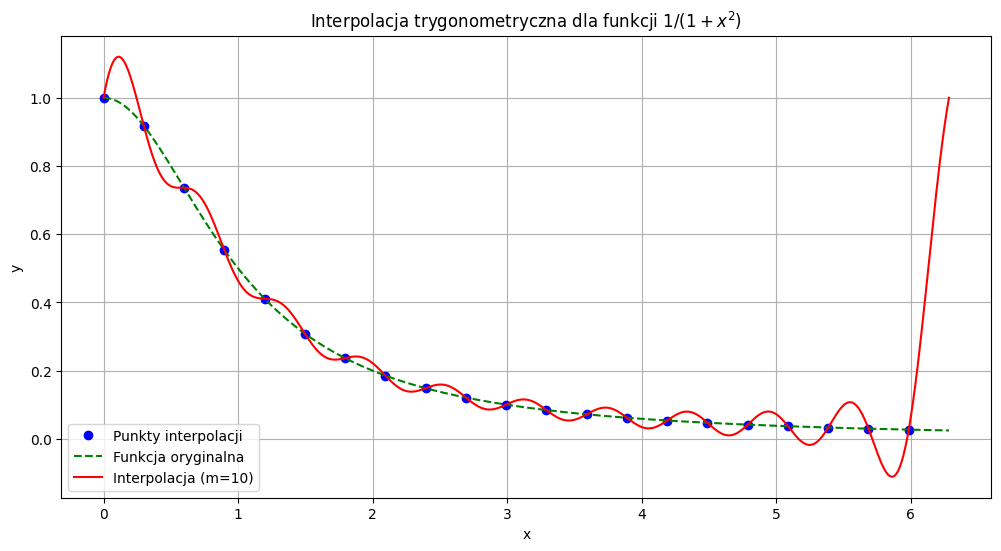
\includegraphics[width=\textwidth]{figures/task-5/rational_10.png}
\end{minipage}
\begin{minipage}{0.49\textwidth}
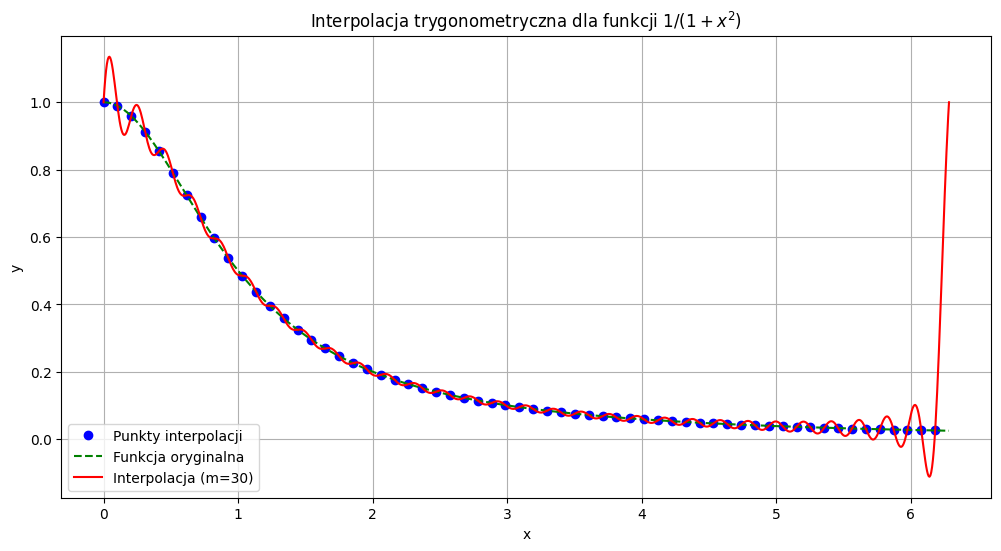
\includegraphics[width=\textwidth]{figures/task-5/rational_30.png}
\end{minipage}

\begin{center}
\textbf{Floor-function results:}
Minimum error: \( 6.00e+00 \),
achieved for \( m = 99 \).
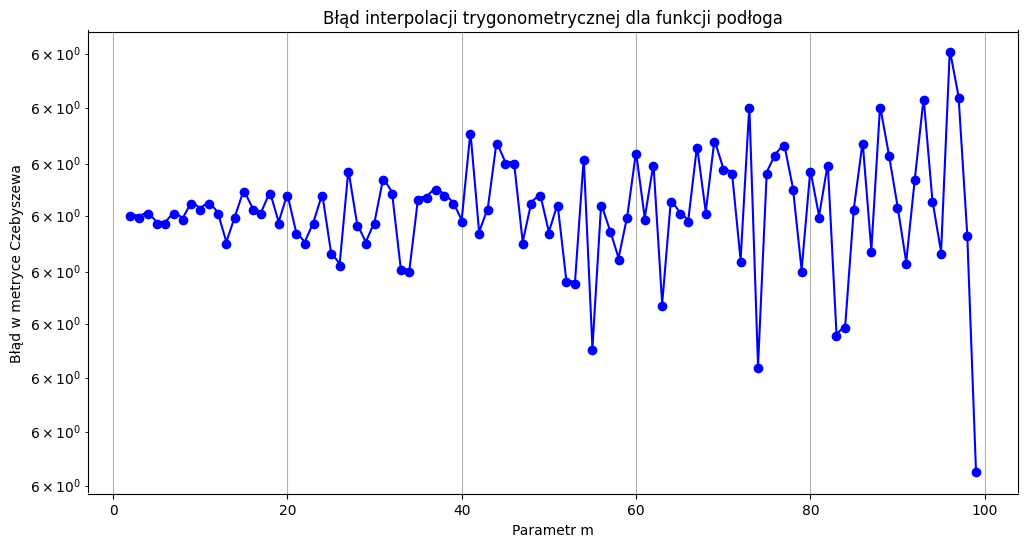
\includegraphics[width=0.8\textwidth]{figures/task-5/floor_error.png}
\end{center}

\begin{minipage}{0.49\textwidth}
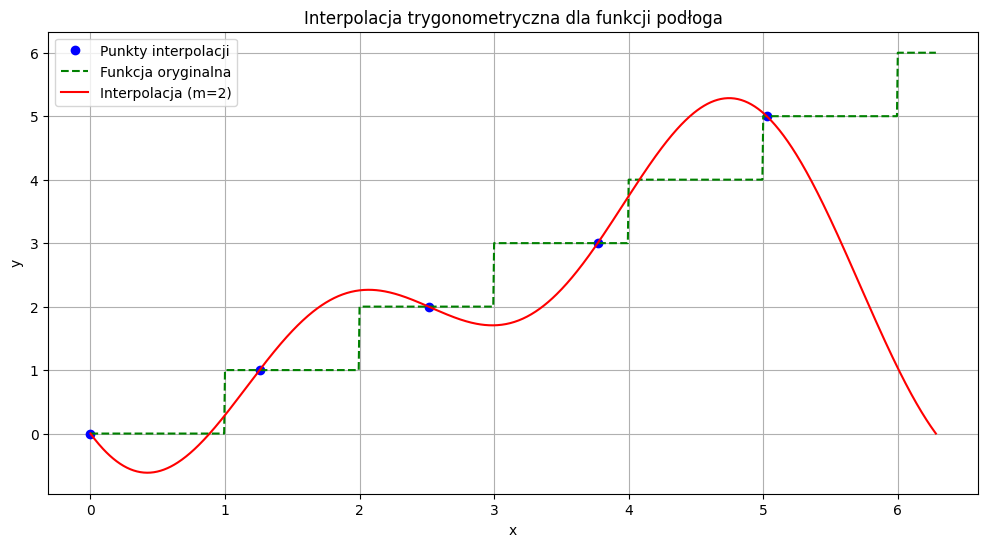
\includegraphics[width=\textwidth]{figures/task-5/floor_2.png}
\end{minipage}
\begin{minipage}{0.49\textwidth}
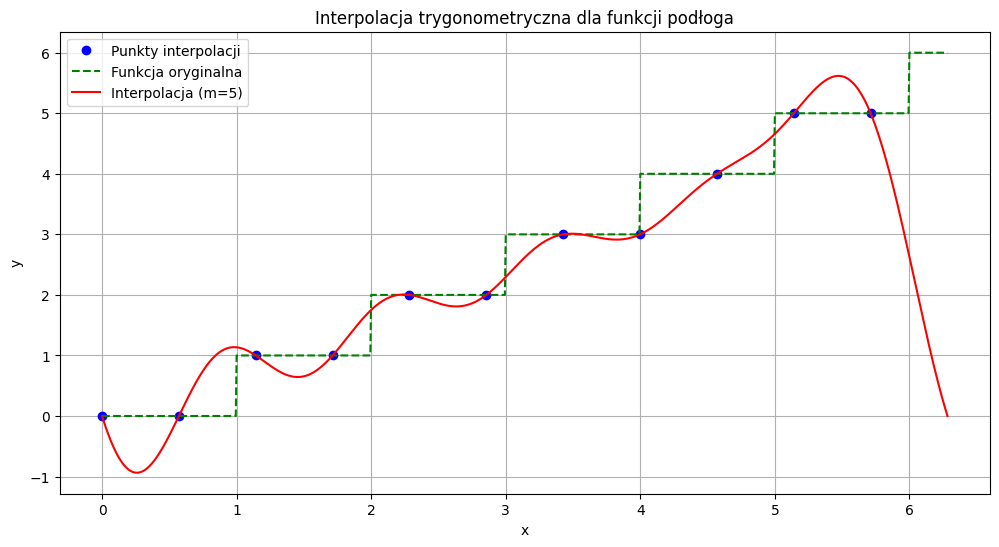
\includegraphics[width=\textwidth]{figures/task-5/floor_5.png}
\end{minipage}

\begin{minipage}{0.49\textwidth}
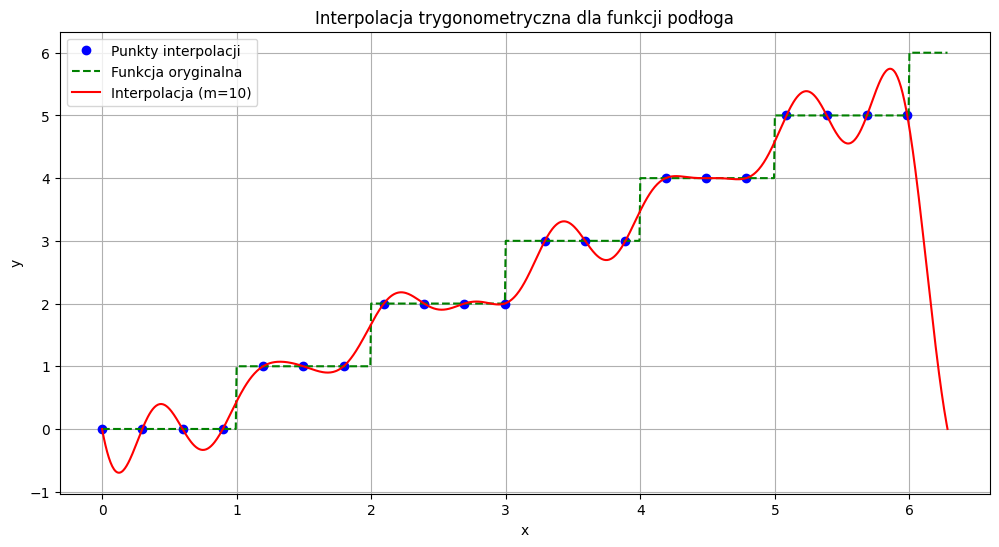
\includegraphics[width=\textwidth]{figures/task-5/floor_10.png}
\end{minipage}
\begin{minipage}{0.49\textwidth}
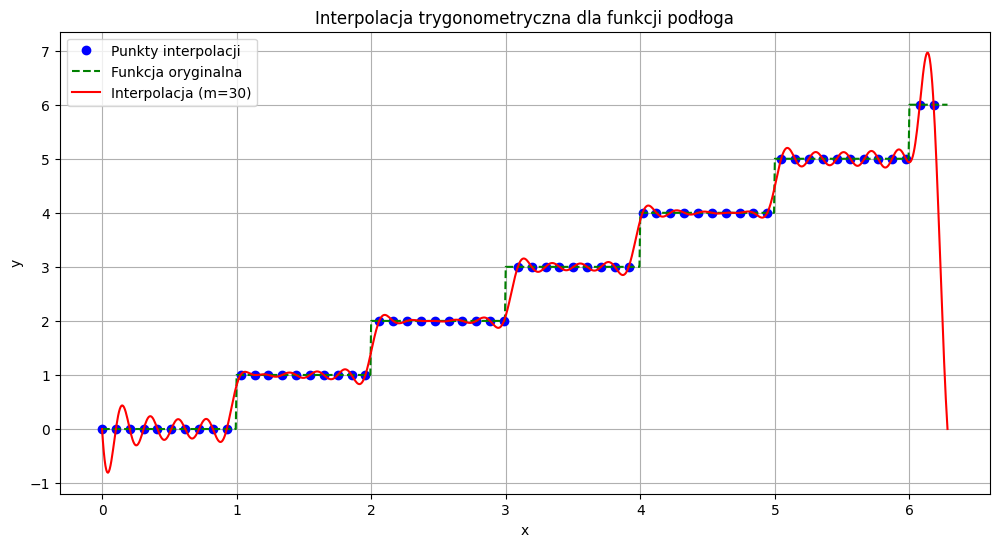
\includegraphics[width=\textwidth]{figures/task-5/floor_30.png}
\end{minipage}

\textbf{Conclusions:}
\begin{itemize}
    \item \textbf{Accuracy:} Trigonometric interpolation gives very small errors for periodic functions such as \( \sin(x) + \cos(x) \).
    \item \textbf{Discontinuous functions:} The algorithm can interpolate discontinuous functions, such as the floor function, although their errors are much larger.
    \item \textbf{Endpoint deviations:} Fluctuations at the ends of the error plots arise from implementation imperfections that could be corrected. In theory, the method should produce the expected results.
    \item \textbf{General applicability:} Scaling the domain to \( [0, 2\pi] \) makes the method applicable to many function types.
\end{itemize}


